\chapter{Multiple Device Activation}\label{chap:MDA-CCRC}
So far the CCRC-solution has been developed with the assumption that devices can only be activated one at a time if they are not part of a network.
The effect of this assumption is that there is no chance of multiple networks being created in range of each other, and there is no chance for two or more devices jamming each other while attempting to connect to an established network.
In this chapter this assumption is removed and the complications this brings will be solved in two sections; one pertaining to the issue that occurs if no network exists i.e. creating of multiple networks, and another pertaining to the issue that occurs if a network already exists i.e. multiple devices simultaneously attempting to connect to an established network.
\section{Multiple Start-up Issue}\label{sec:MSI-CCRC}
%The activation of multiple devices at any point in time such that two or more devices are active but not in a network causes a problem that must be handled differently for each of the two aforementioned cases.
The first case, handled in this section, is in the case where no network exists prior to the activation of devices.
As it has been established earlier, the time required to guarantee no network exists is $\delta \times 3$.
From the moment a device has determined that no network exists, it spends $\delta$ time to announce the existence of a network.
As such if several devices are activated within $\delta$ time, relative to the firstly activated device, multiple networks will be established.
By this it follows that if one can guarantee that devices start with an offset of at least $\delta$ the problem is solved for every case.
In an effort to solve this problem several different approaches can help, however none of them can guarantee that a multiple of networks will never occur with 100 \% certainty. 
As such implementing concepts from several of the following approaches may yield the best result.

\subsection{Definite Solutions}
Firstly definite solutions will be described.
These solutions are easy to check for errors as the result of any operation is predictable, as this limits the statespace to the amount of start configurations possible.

\subsubsection{Unique Offset}
Unique offset is when each device listens for a network for a uniquely specified amount of $\delta$ rather than the initial wait time of $\delta \times 3$.
Using the ID of each device one could guarantee that no device used the same multiple of $\delta$ prior to establishing their network by the formula $\text{\textit{initial wait time}} + \delta \times ID$.

This however assumes device are activated either simultaneously or continuously with rising addresses for it to work.
In the case where initially the device with ID 2 is turned on and exactly $\delta$ time later the device with ID 1 is turned on they would still both create a network, as such this is not a valid solution in itself to the problem.
However this approach could significantly increase the chance of only creating only one network in situations where all the devices are started simultaneously, e.g. a scenario where a multiple of devices are connected to the same power grid, which is then turned off and on again.
Hereby making it appropriate for a uniform start-up process.

\subsubsection{Kill the Network (Definite)}\label{KtN}
If a device is alone in a network for too long it may decide to kill the current network and start listening again.
This works as a recovery technique, allowing two networks to be established but then solving that very problem.
The technique has the network disassemble itself once some factor determines it needs to.

This factor could be when a number of frames has passed without hearing from any other device.
For this to actually work there would have to be implemented something which guarantees that networks would not follow the same pattern, as that could result in a loop of killing and creating networks.
Another problem that occurs is that if more than two networks are created, for this to work all but one network must die within two frames due to the previously set time spent listening.
For the random version it would work similarly to random create, except the outcome would be killing the network rather than creating one.

\subsection{Stochastic Solutions}
The definite solutions could be used, but there will always be a chance for ending up in an infinite loop.
In order to avoid that a random factor is introduced.
With the a stochastic approach whether or not the network is established is now based on probability.
This does not guarantee that a network is never established it is however extremely improbable but not impossible.

\subsubsection{Randomly Create}\label{RCreate}
Once a device is done listening for a network it either creates its own network or resets and starts listening again.
For this each device would need to implement a chance factor to determine whether or not to create a network.
This could be determined by running an algorithm on the result of a random seed, depending on how the algorithm is designed one can obtain whichever chance is preferred.

The problem with this is while it gives the opportunity for two devices to start within the same time-slot without both creating a network at the same time, this is no guarantee; as such this would further require the implementation of a recovery method much like unique offset would.

\subsubsection{Kill the Network (Stochastic)}\label{KtNR}
A version of kill the network could be implementet using a random chance to kill the network if the device is alone.
This would avoid the problem of multiple devices following the same patteren.
As the patteren would be random a soulution is inevitable given enough tries.
The same is true for more than two networks trying to create a network.
At some point an isolated network should exist.

\subsection{Exponential Backoff} 
Using the idea of an increasing exponent, similarly to the technique in exponential backoff as described in \myref[name]{sec:exponential_backoff} can be applied to randomly create, killing the network and unique offset to increase odds of success.

\subsubsection{Kill the Network (Exponential Backoff)}
Once again the random solution here would be implemented similarly to randomly create.
For the non-random deterministic approach the unique factor chosen would be altered exponentially.
A complication in doing so would be that networks would be active for exponential lengths of time, and with the specific requirement of networks having to die within two frames it could worsen the time it takes to successfully establish a single network exponentially; for this reason one might consider using another factor to guarantee unique outcomes for each device, such as an exponential change in listening time which might also be uniquely offset, which also solves the problem with the two frames limitation.

\subsection{Modifications to the Upstart Phase}                 
Based on the aforementioned possibilities a new upstart phase have been designed which minimises the probabilities of devices creating several networks.
The changes are explained in the following text, as well as in the flowchart in \myref{fig:pseudo_flowMultiStart} representing the new design.

\begin{description}[labelindent=\parindent]
    \item[Search for network]\hfill\\
    The initial action after starting a device states to search for a network.
    This is done for $\text{\textit{initial wait time}} + \delta \times b$ where $b$ denotes a random number chosen using the method of exponential backoff from \myref[name]{sec:exponential_backoff}, i.e. $b \in [0, 2^c-1]$, where $c$ is the number of attempts of creating a network.
    This expression ensures that devices will not listen for the same amount of time when they are started, and this difference will increase with each attempt, ensuring the existence scenarios in which only one device will create a network while others are still listening, also in the case where they died at the same time.
    \item[Chance of creating a network]\hfill\\
    This method will not be used in order to keep the method of handling multiple start-up deterministic.
    \item[Alone in network?]\hfill\\
    For this decision the device checks whether or not it is alone in the network; if it is an altered version of \textsc{MainLoop()} is run, making use of the kill network method depending on the result of \textbf{Time to Die?}, as two or more networks could be jamming each other.
    \item[Time to Die?]\hfill\\
    This decision is completely random based on a given chance of killing the device.
\end{description}

\tikzfigure{PseudoFlowDiagramMultiStart}{Revised flow diagram showing how a device acts during the Initialization phase if no networks are detected.}{pseudo_flowMultiStart}


\subsection{Changes to the Pseudocode}
This section will cover the new pseudocode which must be written for those areas multiple startup affects; in \myref{lst:setupCCRC} only five lines handle the creation of a new network, which is line 5 and lines 34-38.
As is shown on the flow diagram \myref{fig:pseudo_flowMultiStart} the multiple network establishment issue is handled with an altered main loop, as such much of the new pseudocode will resemble pseudocode from \myref{lst:general_case}.
The procedure seen in \myref{lst:networkMultiStartCCRC} replaces lines 34 through 38 in \myref{lst:setupCCRC}.
\begin{figure}
\begin{lstlisting}[label=lst:networkMultiStartCCRC,style=pseudocode,mathescape=true,caption={Pseudocode example of the procedure initializeNetwork() for CCRC for the multiple device activation problem.}]
procedure initializeNetwork()
    // Initialize variables
    $x \leftarrow 0$
    $n \leftarrow 2$
    $k \leftarrow 1$
    $i \leftarrow 0$
    $f \leftarrow 0$
    if $firstNetwork \neq \bot$ then
        $a \leftarrow 0$
    end
    
    loop forever       
        run userCode() until $x \geq \delta_{proc}$
        $i \leftarrow (i \text{ mod } n) + 1$ // Update current slot
        if $i = k$ then
            makePayload() //Updates the data to be sent
            transmit($i$, $n$, $id$, $data$)
            if $f < id + C$ then //Time to die check
                $a \leftarrow a + 1$
                $n \leftarrow 0$
                $k \leftarrow 0$
                $f \leftarrow 0$
                $i \leftarrow 0$
                goto $\text{``initialize''}$
            else
                $f \leftarrow f + 1$
            end
        else
            while $x \leq \delta$ do
                if received($i'$, $n'$, $id'$, $data'$) then
                    protocolMaintance($i'$, $n'$, $|data'|$)
                    userRecieve($id'$, $data'$)
                    if $2 < n$ then //alone or not?
                        goto $\text{``mainLoop''}$
                    end
                end
            end
        end
        wait until $x \geq \delta$
        $x \leftarrow 0$ 
    end
    //Enter main loop
    label: $\text{``mainLoop''}$
    wait until $x \geq \delta$
    $x \leftarrow 0$
    mainLoop()
    //Go back to searching for a network
    label: $\text{``initialize''}$
    $firstNetwork \leftarrow \bot$
    initializeNetwork()
\end{lstlisting}
\end{figure}

\bigskip \noindent
With this new procedure for initializing a network, a few new variables are also introduced, all of which are shown in \myref{tab:locals_wmultistartup}.
Furthermore the variable $t_0$ which determines the minimum time required to determine a time slot no longer holds true, as such a new variable, $t_1$ is introduced which replaces $t_0$ on \myref{lst:setupCCRC} line 5.
Note that this no longer denotes the minimum time required to find a network, as that is now non-deterministic due to jamming networks.
\begin{table}[h]
    {\setlength{\extrarowheight}{1ex}%
    \begin{tabularx}{\textwidth}{l|l|X|l}
        \toprule
        Name                & Type      & Description & Constraint \\
        \midrule
        $C$                 & integer   & A constant ensuring that low address devices do not die too often                 & $5 \leq C \leq 15$      \\
        $f$                 & integer   & A counter for how many frames a device has been alone                             & $0 \leq f$  \\
        $a$                 & integer   & A 0 indexed exponent for how many attempts have been made at creating a network   & $0 \leq a \leq 5$     \\
        $t_1$               & integer   & The time spent searching for a network                                            & $t_1 = 3 \times \delta + id^a \times \delta$     \\
        $firstN$            & boolean   & A boolean value used to determine whether or not it is the first attempt at a network         & $a \neq 0 \land firstN = \top \lor$     \\
                            &           &                                                                                   & $a = 0 \land firstN = \bot$     \\

        \bottomrule
    \end{tabularx}}
    \caption{Additional local variables used to avoid multiple networks.}
    \label{tab:locals_wmultistartup}
\end{table}
\clearpage
\section{Simultaneous Connect} % (fold)
\label{sec:simultaneous_connect}

Another problem arises when two or more devices are started simultaneously while a functioning network is up and running.
If all new devices try to connect in the first empty slot, as they should, they will jam each others messages and neither will be heard.
Moreover the jammed, and jamming, devices will never know that their message was not received by anyone, as there is no way of knowing if one transmission was disrupted or jammed.
A device should always try to connect to a network immediately after starting up, to ensure that in non-jamming situations it is fast.
This also means that jams are bound to happen sooner or later, so some measures must be taken to avoid and recover from such situations.
When it comes to multiple devices trying to simultaneously connect to a network, each devices must be able to handle announce conflicts internally.
However the payload should contain some information, which could be used in the solution of these conflicts.

A combination of the following concepts could provide avoidance and recovery from jamming, in the process of joining a network: 
\begin{description}[labelindent=\parindent]
    \item[Validation]\hfill\\
    We should always validate whether or not the announcement has been heard and accepted by the network (one device under CCRC), before joining the network.
    \item[Payload Mode]\hfill\\
    The header of the payload should contain an extra field, which can indicate different modes or some other variable.
    If the design using modes is chosen, it would be possible for other devices implementing the protocol to do various actions upon the data of the payload, e.g. the mode can indicate that the first byte of the date contains the address of a device, which is allowed to join the network.
    Further explanation will be presented in \myref{ssub:modes_and_validation}
    \item[Exponential Backoff]\hfill\\ 
    If no one in the network responds to a device's announcement, or it is not validated, the device will use exponential backoff in regards to how many frames it should wait before trying again.
\end{description} 
\noindent
Using the concepts above it would be possible to design and implement a strategy for handling a scenario, where two or more devices tries to join the same network simultaneously.
The modifications to the existing design from \myref{cha:Design} needed, will be shown in the following paragraphs.

\subsection{Modification of The Payload} % (fold)
\label{sub:modification_of_the_payload}
To pass around information, which is valuable to the protocol, the payload needs to be modified.
This modification should add information where needed and remove unused information in other cases.
In the following paragraph the specific modification, which is needed to accommodate for simultaneously connecting devices, will be presented. 

\subsubsection{Modes and Validation} % (fold)
\label{ssub:modes_and_validation}
The first modification to the payload, is to introduce a way of indicating modes.
With this addition it is possible to utilise the data part of the payload for auxiliary information, e.g. if the mode indicates a validation payload, the first byte of the data could be the address of the device accepted into the network.
Such a modification with mode in the payload header can be seen on \myref{fig:payloadwMode}, where \emph{mode} is inserted after \emph{Address} and before \emph{Data}. 

\tikzfigure{Payload_wModes.tikz}{Modified payload containing an indicator for mode}{payloadwMode}

\noindent
Along side the possibility of sending validation payloads using modes, other functions could benefit from this in the future, e.g. targeted payloads, payload that should be echoed or other special cases.
% subsubsection modes_and_validation (end)

% subsection modification_of_the_payload (end)

\subsection{Introduction of Exponential Backoff} % (fold)
\label{sub:introduction_of_sub_slots_and_exponential_backoff}
To ensure a faster conflict solving if multiple devices try to connect simultaneously, a two-step process is designed.
These two steps consists of choosing a random offset of sub slots to wait in the empty slot, along with a strategy of exponential back-off if jamming occurs.
On \myref{fig:pseudo_flowMultiConnect} it can be seen how said two-steps is merged into the existing flow chart (\myref{fig:psuedo_flowCCRC}) from \myref{sub:setupCCRC}

\begin{figure}[p]
    \centering \footnotesize
    \tikzstyle{decision} = [diamond, draw, fill=yellow!20, 
    text width=4.5em, text badly centered, node distance=3cm, inner sep=3pt]
\tikzstyle{block} = [rectangle, draw, fill=green!40, 
    text width=6em, text centered, rounded corners, minimum height=4em]
\tikzstyle{line} = [draw, -latex']
\tikzstyle{cloud} = [draw, ellipse,fill=red!20,
    minimum height=2em, align=center]
\begin{tikzpicture}[node distance = 3.8cm, auto]
    % Place nodes
    \node [cloud] (start) {Start};
    \node [block, right of=start] (search) {Search for network};
    \node [decision, below of=search] (found) {Found network?};
    \node [cloud, left of=found] (init) {GOTO \\ init network};
    \node [block, below of=found] (listen) {Listen while waiting for empty slot};
    \node [block, right of=listen] (announce) {Announce in the empty slot, using a random offset};
    \node [decision, below of=listen] (validated) {Validated?};
    \node [block, right of=validated] (listenvalidate) {Listen for validation from the network};
    \node [block, left of=validated] (expbackoffcalc) {Determine an exponential backoff}; 
    \node [block, left of=listen] (backoff) {Wait for back-off amount of frames}; 
    \node [block, below of=validated] (join) {Take k after what the empty slot had}; 
    \node [cloud, left of=join] (mainloop) {GOTO \\ main loop};

    % Draw edges
    \path [line] (start) -- (search);
    \path [line] (search) -- (found);
    \path [line] (found) -- node {no} (init);
    \path [line] (found) -- node {yes} (listen);
    \path [line] (listen) -- (announce);
    \path [line] (announce) -- (listenvalidate);
    \path [line] (listenvalidate) -- (validated);
    \path [line] (validated) -- node {no} (expbackoffcalc);
    \path [line] (validated) -- node {yes} (join);
    \path [line] (expbackoffcalc) -- (backoff);
    \path [line] (backoff) -- (listen);
    \path [line] (join) -- (mainloop);  
\end{tikzpicture}                                   
    \caption{Revised flow diagram showing how a device acts during the Initialization phase}
    \label{fig:pseudo_flowMultiConnect}
\end{figure}

The flow chart in \myref{fig:pseudo_flowMultiConnect} shows that the random offset of sub slots is the first method of prevention when it comes to simultaneous connection of multiple devices.
If a device hears another announcement before it has sent it's own in the chosen sub slot, it will abort the announce-phase and wait for the next empty slot before trying immediately again.
However if a device announces it self and does not get validated by the network, because the announcement was jammed, it will use exponential backoff to prevent further collisions.

\subsubsection{Exponential Backoff} % (fold)
\label{ssub:exponential_backoff}
The method of exponential backoff to be used here consists of:
\begin{enumerate*}[label=\itshape \alph*\upshape)]
    \item remembering how many unvalidated announcements have been sent, this will typically be caused by collisions; and
    \item choosing a random number of frames to wait based upon this number.   
\end{enumerate*}
These properties of the exponential backoff can be expressed as follows:
\begin{equation}
     x \in [0, 2^c - 1] \mid x \in \mathbb{Z}^+, c \in [1,5]
\end{equation}
Where $x$ is a randomly chosen number of frames to wait from the range, and $c$ is number of unvalidated announcements. With this method a device will wait 0 to 1 frames after the first unvalidated announcement, 0 to 3 after the second and 0 to 7 after the third. To avoid an infinite increase of the wait time the $c$ should have an upper limit of e.g. 5, which would ensure a maximum wait of $2^5-1 = 31$ frames.

% subsubsection exponential_backoff (end) 
% subsection introduction_of_sub_slots_and_exponential_backoff (end)

\subsection{Changes to the Pseudocode} % (fold)
\label{sub:changes_to_the_pseudocode}
Because the problem of multiple devices connecting simultaneously only exists during the initialisation phase, the change to the pseudocode from \myref{sec:Pseudo} will only affect \myref{sub:setupCCRC}.
Therefore the following modification will focus on line 15-32 (both inclusive) from \myref{lst:setupCCRC}, which deals with what happens if a network is found.
In the modified pseudocode some new variables and constants are introduced, these are presented and explained in \myref{tab:locals_wmulticonnect}.

\begin{table}[h]
    {\setlength{\extrarowheight}{1ex}%
    \begin{tabularx}{\textwidth}{l|l|X|l}
        \toprule
        Name                & Type      & Description & Constraint \\
        \midrule
        $valid$             & boolean   & Indication of validation              \\
        $c$                 & integer   & Number of failed announcements        & $0 \leq c \geq c_{max}$ \\
        $c_{max}$           & integer   & Ceiling of $c$                        \\
        $b$                 & integer   & Number of frames to wait              & $b \in [0, 2^c-1]$ \\
        \bottomrule
    \end{tabularx}}
    \caption{Additional local variables every device has access to.}
    \label{tab:locals_wmulticonnect}
\end{table}

The modified pseudocode is significantly more complex than the previous verison of the connecting phase.
This is the case because of the two-step strategy previously discussed, which requires addition of several looping and conditional constructs.
In \myref{lst:pseudoInitMulti} the 17 lines from \myref{lst:setupCCRC}, which concerned connecting, have been expanded to 54 lines of code. 

\begin{algorithm}[h]
\caption{Modified section of initialise procedure for when network found.}
\label{lst:pseudoInitMulti}
\begin{algorithmic}[1]
\Require $c$ is initialised
\Procedure {ConnectToNetwork}{ }
    \While {$i \neq n$}
        \State \textbf{run} \Call{UserCode}{ } $\text{ \textbf{until} }x \ge \delta_{proc}$ 
        \State $i \gets (i \bmod n) + 1$
        \While {$x \le \delta$}
            \If {\Call{Received}{$i', n', id', mode', data'$}}
                \State \Call{ProtocolMaintenanca}{$i', n', |data'|$}
                \State \textbf{break}
            \EndIf
        \EndWhile
        \State \textbf{wait until } $x \le \delta$
        \State $x \gets 0$
    \EndWhile
    \State \Call{Transmit}{$i, n, id, data$} \Comment{Send announcement}
    \State $x \gets 0,\, i \gets 0,\, valid \gets \bot$
    \While {$i \neq n$}
        \State \textbf{run} \Call{UserCode}{ } $\text{ \textbf{until} }x \ge \delta_{proc}$
        \State $i \gets (i \bmod n) + 1$
        \While {$x \le \delta$}
            \If {\Call{Received}{$i', n', id', mode', data'$}}
                \State \Call{ProtocolMaintenanca}{$i', n', |data'|$}
                \If {\Call{Validated}{$mode', data'$}}
                    \State $valid \gets \top$
                \EndIf
            \EndIf
        \EndWhile
        \State \textbf{wait until } $x \le \delta$
        \State $x \gets 0$ 
    \EndWhile
    \If {$valid$}
        \State $k \gets n$ \Comment{Obtain timeslot}
        \State \Call{MainLoop}{ }
    \Else
        \If {$c < c_{max}$}
            \State $c \gets c+1$
        \EndIf
        \State $b \gets \text{random } \in [0, 2^c -1]$
        \While {$b > 0$}
            \State \textbf{wait} $1 \text{ frame}$
            \State $b \gets b - 1$
        \EndWhile
        \State \Call{ConnectToNetwork}{ }
    \EndIf
\EndProcedure
\end{algorithmic}    
\end{algorithm}

% subsection changes_to_the_pseudocode (end)

% section simultaneous_connect (end) 
\newpage
\section{Statistical Model Checking}

When a model rely on stochastic behaviours, such as randomness, its state-space grows exponentially (sometimes called a state-space explosion) therefore an exhaustive search determining whether if some property holds is not possible in reasonable time. 
Instead one can estimate a percentage chance a property holds, within a given probability of uncertainty, with a Statistical Model Chcker (SMC). 

%UPPAAL SMC Explanation
\subsection{UPPAAL SMC}
\begin{wrapfigure}[18]{r}{0.3\textwidth}
\centering
  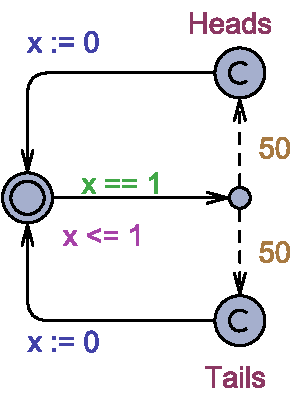
\includegraphics[width=0.3\textwidth]{Figures/Model/Simple_SMC.pdf} 
\caption{A simple UPPAAL SMC model with weighted edges. }
\label{fig:simpleSMC}
\end{wrapfigure}

To do this in UPPAAL there is an extension called UPPAAL SMC, a full tutorial is available here ``Uppaal SMC Tutorial''\cite{DBLP:journals/sttt/DavidLLMP15} by Alexandre David, Kim G. Larsen, Axel Legay, Marius Miku\v{c}ionis, Danny B\o gsted Poulsen.

In UPPAAL SMC there is a new type of edge, this is a weighted edge and is shown as a dashed line. 
An example of this can be seen in figure \myref{fig:simpleSMC}. 
The figure shows a simple UPPAAL SMC model, following the initial state there is a ``branch point'' from which there are two weighted edges.
The number by the weighted edges give their probability of being taken, this simple concept allows UPPAAL SMC to do randomness without having to explore the full state-space, as it can run simulations taking each edge a number of times corresponding to their weights. 
This example simulates a coin toss, giving 50 \% chance of heads and 50 \% chance of tails. 

UPPAAL SMC can additionally draw several types of plots which shows what the chance of a given query being true after a given run duration.

It is possible to set the statistical parameters for UPPAAL SMC, such as: Probability uncertainty, Probability of false negatives and Probability of false positives. 
Setting these parameters closer to zero will cause the time it takes to verify a query for a model to increase drastically, however it will also be more accurate. 

%Description of changes to the model in UPPAAL

\subsection*{Changes to the model}

\info[inline]{Syndes der er meget svag opdeling i dette afsnit, man kunne lave en subsub med ``Removing assumptions'', ``multi-start changes'', ``multi-connect changes'' - Troels}

The UPPAAL model shown in \myref{sec:themodel} has gone through extensive changes to accomodate the challenges posed of multiple devices starting at the same time.
The complete model can be seen in the back of the project report printed on a A3-paper, and it can also be found on the CD, which is also in the back of the project folder.

\paragraph{Jamming} can now occur since multiple devices are turned on at the same time, which means that more than one device is now able to transmit at the same time.
If two or more devices transmit at the same time, i.e. a jam, then none of the receiving devices will be able to receive any payloads, this is also mentioned in \myref{subsubsec:RadioHead}, this needs to be modelled in UPPAAL. 
%When this happens, it has been mentioned in \myref{subsubsec:RadioHead}, that nothing is detected by the receivers, therefore a mechanism making sure that when two devices are trying to transmit at the same time, nothing will be received by anyone are needed in UPPAAL. 

\paragraph{Multiple Startup.}
In the previous model presented in \myref{sec:themodel} only one device was able to start at a time, as there was nothing to handle multiple starting at the same time.
\begin{wrapfigure}[18]{r}{0.5\textwidth}
\centering
  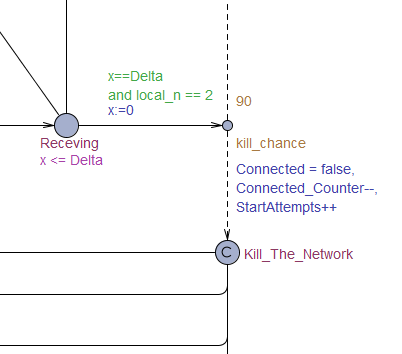
\includegraphics[width=0.5\textwidth]{Figures/Model/Screenshot_Of_Kill.png} 
\caption{Graph showing the split node after not receiving, where there is a chance for the device to start over and kill the network.}
\label{fig:Screenshot_Of_Kill}
\end{wrapfigure}

This limitation will be removed in this model.
%The devices can now start at the same time again, as was possible before the mechanism controlling when a device was released was implemented, as presented in \myref{sec:verifyingTheModel}.
To stop devices from being alone in a network forever, a split node is made when nothing is received in a time slot, where the device is alone in the network, i.e. the \texttt{local\_n} of the device is equal to 2.
This split node has 2 outgoing edges, one edge which has a probability weight of 90, which makes the device go back into its main loop, and another edge with a probability of \texttt{kill\_chance} (10 \%), which make the device kill the network, and start listening again.
When this happens the exponential backoff method is used, which means for each time a device kills the network it will have a chance of listening for a longer period of time, according to the specification in the previous sections.
This are the changes needed for the model, in order for the devices to start trying to connect to the same network instead of multiple networks.
\myref{fig:Screenshot_Of_Kill} shows the split node leaving the location after not receiving a transmission.



\paragraph{Multile Devices Connecting.}
The other problem is for when devices try to connect to the same network at the same time.
A verification loop has been created for the model, where all devices which transmitted that they wanted to join the network will listen for the number of devices acknowledging their request of joining the network.
If the amount of acknowledgments are lower than half of the devices in the network, they will also use the exponential backoff method, where they will wait for a random number of frames, in an increasingly larger range, with a cap of 31 frames (It only require one acknowledgment in the CCRC, but this solutions is chosen, to easier expand to CCUC).
This is the only change needed for handling multiple devices connecting to the network, the specifics of the implementation of this on the model will not be presented in this section, but for the curious reader the specifics can be seen in the back as previously mentioned.

%New Queries using SMC

\subsection*{Verifying using SMC}

Some of the queries presented in the previous UPPAAL section, \myref{sec:verifyingTheModel}, make no sense for the new model, as now multiple networks should be running at the same time when the devices first start up, and therefore checking if the value of \texttt{i} is the same for all devices in a certain state makes no sense.
When verifying using SMC then the querys will yield a probability of being true within a given confidence interval, rather than true or false as in the normal UPPAAL.
Therefore the queries will all except for one be checking for the probability of them being true over time, when at least 3000 UPPAAL time units has passed.
The choice of 3000 time units is because this gives enough time for all devices to start up, and at least as some of them should have started a network. 
It should be noted that the model uses time estimates which roughly translate to the time being used in each phase for the hardware used in this project, where a time-slot length is $\delta = 250$.

All the queries have been run with five devices in the system, and a confidence of 0.999.
All queries' cumulative probability is shown on \myref{fig:ConnectQueryTime}.
The first query is the only query which was also used on the earlier model, and it will still give a result indicating the query holds.

\begin{lstlisting}[style=UPPAAL, title={This query requires that eventually if all devices are connected, then no pair of devices have the same \texttt{k}, unless the pair consists of the same two devices. This is true.}]
1. A<> forall(i : id_t) forall(j : id_t) Device(i).Connected and
         Device(j).Connected and Device(i).k == Device(j).k imply i == j
\end{lstlisting}

\begin{lstlisting}[style=UPPAAL, title={This query asks after 3000 UPPAAL time units has passed, what then is the probability that if two devices \texttt{i}, and \texttt{j} are connected to a network that their local values of \texttt{n} are the same, and that they are both connected to the same network. This means that the devices are connected to the same network. UPPAAL runs this query and within 3451 runs [0.998,1] with confidence 99.9 \% this is true. }]
2. Pr[<=300000] ( <> forall(i : id_t) forall(j : id_t) (time > 3000) 
    and (Device(i).Connected and Device(j).Connected 
    imply ((Device(i).local_n == Device(j).local_n)
        and Device(i).local_network_id == Device(j).local_network_id)))     
\end{lstlisting}

\begin{lstlisting}[style=UPPAAL, title={This query asks after 3000 UPPAAL time units has passed, what then is the probability that if a device \texttt{i} and a device \texttt{j} is both connected that then \texttt{i}'s values of \texttt{k} will be larger than zero and smaller than any \texttt{n}, and that they are connected to the same network. This query insures that all the \texttt{k}-values are within the wanted range after a network is made. UPPAAL runs this query and within 3451 runs [0.998,1] with confidence 99.9 \% this is true.}.]
3. Pr[<=300000] ( <> forall(i : id_t) forall(j : id_t) (time > 3000) 
    and (Device(i).Connected and Device(j).Connected 
    imply (Device(i).k < Device(j).local_n and Device(i).k > 0) 
        and Device(i).local_network_id == Device(j).local_network_id))

\end{lstlisting}

\begin{lstlisting}[style=UPPAAL, title={This query asks after 3000 UPPAAL time units has passed, what then is the probability that a device \texttt{i} has a local value of \texttt{n} to be equal to the number of devices plus the the empty slot, which is \texttt{N} + 1, which means that all devices are in the same network. UPPAAL runs this query and within 3451 runs [0.998,1] with confidence 99.9 \% this is true.}]
4. Pr[<=300000] Pr[<=300000] ( <>  forall(i : id_t) (time >3000) 
    and Device(i).local_n == N + 1)
\end{lstlisting}

\begin{lstlisting}[style=UPPAAL, title={This query is a generalisation of the previous which includes a check of whether when one device finish transmitting then the rest are just finished receiving. UPPAAL runs this query and within 3451 runs [0.998,1] with confidence 99.9 \% this is true.}]
5. Pr[<=300000] ( <>  forall(i : id_t) forall(j : id_t) (time >3000) 
    and (Device(i).local_n == N+1) 
    and (Device(i).Done_Transmitting 
    imply (Device(j).Just_Received or i==j)))
\end{lstlisting}

%GRAPHS

\begin{figure}[ht]
  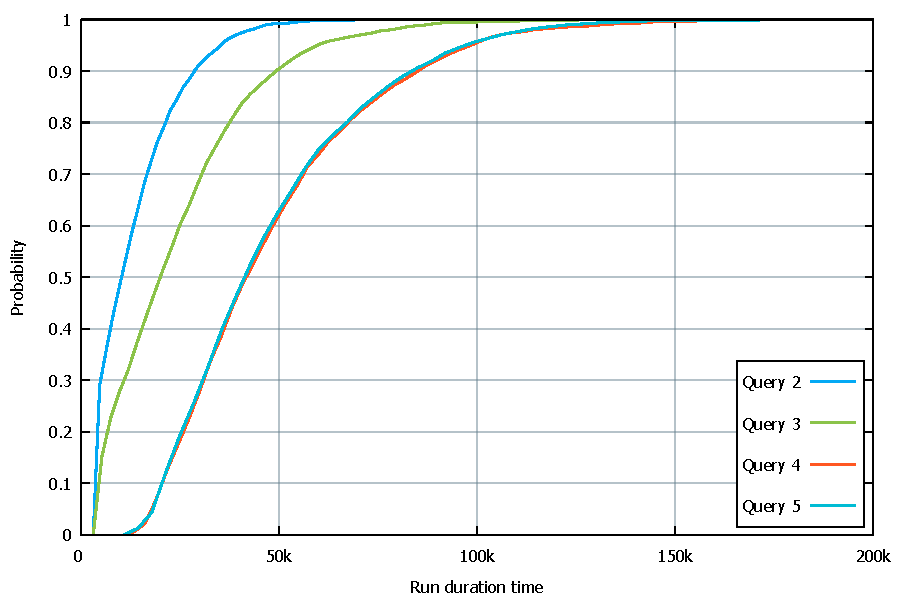
\includegraphics[width=1\textwidth]{Figures/Graphs/gnuplot/uppaal/graph.pdf} 
\caption{Graph of the UPPAAL SMC queries, in which the cumulative probability increase over time.}
\label{fig:ConnectQueryTime}
\end{figure}

\todo{Redo this graph.}

As can be seen the change in probability approaches one as time increases, and appears to be a logarithmic growth, and will according to UPPAAL eventually connect, however it might take some time for it to do so.
This is because in the worst case the random numbers generated will keep causing collisions, or maybe they will take a long time before eventually killing their networks.
There are many possible explanations for what causes the longer runs, but it it important to note the fact that, the longer the devices are running the bigger the chances are of establishing a stable network.


\section{Conclusion}
This chapter presented a way to handle the startup of multiple devices, which made use of the method exponential backoff, which results in an increasingly randomly generated number of wait time for the devices. 
The randomness results in all devices eventually becoming connected to the network since they will be split up and thus stop jamming each other.
The UPPAAL model created data, which can be seen on \myref{fig:ConnectQueryTime}.
The data shows that the Arduinos will eventually be connected to the same network, however it does take some time, approximately $150 000$ UPPAAL time units.
This means that an implementation of this design should be able to solve the issues of turning on more Arduinos at the same time, assuming our assumptions are correct.


